%\section{Data}


The Named Entity Disambiguation is performed on articles of historical newspapers obtained from Chronicling America\footnote{\texttt{http://chroniclingamerica.loc.gov/}}. The newspapers are scanned on a page-by-page basis and article level
segmentation is performed by human annotators. Articles of ``The Sun" newspaper from November-December 1894 consisting of 14020 news articles are used in our study. 
The Optical Character Recognition (OCR) scanning process used to convert historical newspaper pages into machine recognizable text is far
from perfect and the documents generated from it contain a large
amount of garbled text.
An individual OCR text article has at least one or more of the following types of spelling errors:
 \textbf{1) Real word errors} include words that are spelled correctly in the OCR text but still incorrect when compared to the original newspaper article image.  \textbf{2) Non-real word errors} include words that have been misspelled due to some insertion, deletion, substitution or transposition of characters from a word.  \textbf{3) Non-word errors} include words that have been spelled incorrectly and are a combination of alphabets and numerical characters. \textbf{4) New Line errors} include words that are separated by hyphens where part of a word is written on one text line and remaining part in the next line. 
\textbf{5) Word Split and Join errors} include words that either get split into one or more parts or some words in a sentence get joined to a make a single word. 
For example, in Figure~\ref{figure:1} the word ``coil"  has been correctly spelled in the OCR text but should have been ``and" according to the original newspaper article (real word error); the word ``tnenty" in the OCR text has a substitution error (`n' should have been `w') which is actually ``twenty" according to the original newspaper article (Non-real word error); the word ``4anrliteii" is a combination of alphabets and number and should have been ``confident" as per the original newspaper article(Non-word error); the word ``ex-ceptionally" where ``ex" occurs on one line while ``ceptionally" in the next and due to no punctuation in the text, they are treated as separate words in OCR text(New Line error); the word ``Thernndldntesnra" in the OCR text is actually a combination of three words ``The candidates are" while the words ``v Icrory" are actually equivalent to a single word ``victory" when compared with the original news article(Word Split and Join error).

%This is an
%initiative of the National Endowment for Humanities (NEH) and the
%Library of Congress (LC) whose goal is to develop an Internet-based, searchable database of U.S. newspapers(between
%1836 and 1922) with descriptive information and select digitization of historic pages. 
%Under this program, institutions such as libraries receive an award to select and digitize approximately 100,000 newspaper pages representing that state's regional history, geographic coverage, and events of the particular time period being covered. The scanned newspaper holdings of the New York Public Library are a source of prosopographical studies. 

\begin{figure*}
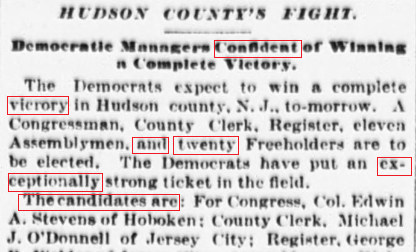
\includegraphics[scale=0.75]{originalimage}
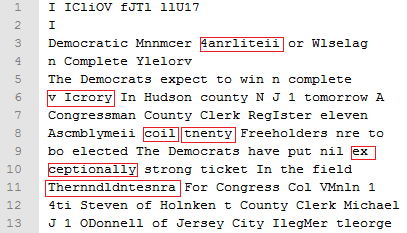
\includegraphics[scale=0.80]{ocr}
\caption{Scanned Image of a Newspaper article (left) and its OCR raw text (right)}
\vspace{-10pt}
\label{figure:1}

\end{figure*}

%\subsection{Characteristics}


%\begin{itemize}
 %\item \textbf{Real word errors}	 include words that are spelled correctly in the OCR text but still incorrect when compared to the original newspaper article image. For example: In Figure~\ref{figure:1}, the word ``coil"  has been correctly spelled in the OCR text  but should have been ``and" according to the original newspaper article. 
 %\item \textbf{Non-real word errors} include words that have been misspelled due to some insertion, deletion, substitution or transposition of characters from a word. For eg. In Figure~\ref{figure:1}, the word ``tnenty" in the OCR text has a substitution error (`n' should have been `w') which is actually ``twenty" according to the original newspaper article.
 %\item \textbf{Non-word errors} include words that have been spelled incorrectly and are a combination of alphabets and numerical characters. For example: In Figure~\ref{figure:1}, the word ``4anrliteii" is a combination of alphabets and number and should have been ``confident" as per the original newspaper article.
%\item \textbf{New Line errors} include words that are separated by hyphens where part of a word is written on one text line and remaining part in the next line. For example: In Figure~\ref{figure:1}, the word ``ex-ceptionally" where ``ex" occurs on one line while ``ceptionally" in the next and due to no punctuation in the text, they are treated as separate words in OCR text.
%\item \textbf{Word Split and Join errors} include words that either get split into one or more parts or some words in a sentence get joined to a make a single word. For example: In Figure~\ref{figure:1}, the word ``Thernndldntesnra" in the OCR text is actually a combination of three words ``The candidates are" while the words ``v Icrory" are actually equivalent to a single word ``victory" when compared with the original news article.
%\end{itemize} 

%\subsection{Statistics}
%The OCR text available from Chronicling America website is on a page by page level and no article level segmentation is provided. OCR text dataset is therefore, taken from a PostgreSQL database where 
%A total of 8,403,844 tokens are generated from a bag-of-words extraction. 
%The newspaper database ER diagram \footnote{https://power.ldeo.columbia.edu/twiki/pub/Incubator/BodhiDBDesign/Final ERD.pdf }
%is used to extract the required articles text from the database by dumping complete dataset and extracting individual articles linetext based on their unique ID. 
%The text from the articles do not have any punctuation and contain a large amount of garbled text containing above mentioned OCR errors.


